\documentclass{article}
\usepackage{fullpage,abstract,hyperref,graphicx,caption}
\usepackage{amsmath,amsfonts,amssymb,amsthm,program,float,multirow}

\makeatletter

\newfloat{algorithm}{thp}{lop}
\floatname{algorithm}{Algorithm}

\title{\vspace{-60pt}CS 6491 - Project 2 - Delaunay Triangulation}
\date{}
\author{
\begin{tabular}{ll}
\multirow{3}{*}{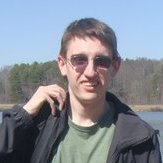
\includegraphics[scale=0.4]{chris.jpg}}\\&
Christopher Martin\\&\texttt{chris.martin@gatech.edu}\end{tabular}
~\\~\\~\\}

\newcommand\photo[3]{
  \centering
  \includegraphics[width=80pt]{#1}
  \\\textbf{#2}\\[2pt]\texttt{\small#3}\\[5pt]
}

\begin{document}

\makeatletter
\twocolumn[
\begin{@twocolumnfalse}
\maketitle

\begin{abstract}

In this project I build a Delaunay triangulation from a set of
randomly-generated vertices

\end{abstract}
\end{@twocolumnfalse}
]
\makeatother

% \begin{figure}
% \centering
% \screenshot{init}
% \caption{A game's starting configuration.}
% \end{figure}

\end{document}

